\section{Evaluation}
\label{sec:evaluation}

We evaluate guided proofreading on multiple different real-world connectomics datasets of different species. All datasets were acquired using either serial section electron microscopy (ssEM) or serial section transmission electron microscopy (ssTEM). We perform experiments with the selection oracle, with automatic selection with threshold, and in the forced choice setting via a between-subjects user study with both novice and expert participants.

\subsection{Datasets}

\paragraph{L. Cylinder.} We use the left part of the 3-cylinder mouse cortex volume of Kasthuri \etal~\cite{kasthuri2015saturated} ($2048\times2048\times300$ voxels). The tissue is dense mammalian neuropil from layers 4 and 5 of the S1 primary somatosensory cortex, acquired using ssEM. The dataset resolution is $3\times3\times30~\text{nm}^3\text{/voxel}$. Image data and a manually-labeled expert `ground truth' segmentation is publicly available\footnote{\scriptsize{\url{https://software.rc.fas.harvard.edu/lichtman/vast/}}}.

\paragraph{AC4 subvolume.} This is part of a publicly-available dataset of mouse cortex that was published for the ISBI 2013 challenge ``SNEMI3D: 3D Segmentation of neurites in EM images''. The dataset resolution is $6\times6\times30~\text{nm}^3\text{/voxel}$ and it was acquired using ssEM. Haehn~\etal~\cite{haehn_dojo_2014} found the most representative subvolume ($400\times400\times10$ voxels) of this dataset with respect to the distribution of object sizes, and used it for their interactive connectomics proofreading tool experiments. We use their publicly available data, labeled ground truth, and study findings\footnote{\scriptsize{\url{http://rhoana.org/dojo/}}}.

\paragraph{Automatic segmentation pipeline.}
We use a state-of-the-art method to create a dense automatic segmentation of the data. Membrane probabilities are generated using a CNN based on the U-net architecture (trained exclusively on different data than the GP classifiers)~\cite{RonnebergerFB15}. The probabilities are used to seed watershed and generate an oversegmentation using superpixels. Agglomeration is then performed by the GALA active learning classifier with a fixed agglomeration threshold of 0.3~\cite{nunez2014graph}. We describe this approach in the supplemental material.

\subsection{Classifier Training}

We train our split error classifier on the L. Cylinder dataset. We use the first 250 sections of the data for training and validation. For n-fold cross validation, we select one quarter of this data and re-select after each epoch. We minimize cross-entropy loss and update using stochastic gradient descent with Nesterov momentum~\cite{nesterov}. To generate training data, we identify correct regions and split errors in the automatic segmentation by intersection with ground truth regions. This is required since extracellular space is not labeled in the ground truth, but is in our dense automatic segmentation. From these regions, we sample 112,760 correct and 112,760 split error patches with 4-channels (Sec.~\ref{sec:spliterrordetection}). The patches are normalized. To augment our training data, we rotate patches within each mini-batch by $k*90$ degrees with randomly chosen integer $k$. The training parameters such as filter size, number of filters, learning rate, and momentum are the result of intuition and experience, studying recent machine learning research, and a limited brute force parameter search (see supplementary material). 

Table~\ref{tab:parameters} lists the final parameters. Our CNN configuration results in 171,474 learnable parameters. We assume that training has converged if the validation loss does not decrease for 50 epochs. We test the CNN by generating a balanced set of 8,780 correct and 8,780 error patches using unseen data of the left cylinder dataset. 

\begin{table}[t]
\caption{Training parameters, cost, and results of our guided proofreading classifier versus focused proofreading by Plaza~\cite{focused_proofreading}. Both methods were trained on the same mouse brain dataset using the same hardware (Tesla X GPU).}
\small{
\begin{tabular}{ll}
	\toprule
	\begin{tabular}{l}
		\textbf{Guided Proofreading} \\ \midrule
		\emph{Parameters} \\ \midrule
		Filter size: 3x3 \\ No. Filters 1: 64 \\ No. Filters 2--4: 48 \\ Dense units: 512 \\ Learning rate: 0.03--0.00001\\ Momentum: 0.9--0.999\\Mini-Batchsize: 128 \\
	\end{tabular}
	&
	\begin{tabular}{l}
		\vspace{0.2mm} \\
		\midrule
		\emph{Results---Test Set} \\ \midrule Cost [m]: 383 \\ Val. loss: 0.0845 \\ Val. acc.: 0.969 \\ Test. acc.: 0.94 \\ Prec./Recall: 0.94/0.94 \\ F1 Score: 0.94 \\ ~ \\
	\end{tabular}
\end{tabular}

\vspace{0.5mm}
\begin{tabular}{ll}
	\toprule
	\begin{tabular}{l}
		\textbf{Focused Proofreading}\\ \midrule
		\emph{Parameters} \\ \midrule
		Iterations: 3 \\
		Learning strategy: 2\\
		Mito agglomeration: Off~~~~~~ \\  
		Threshold: 0.0\\~\\
	\end{tabular}
	&
	\begin{tabular}{l}
		\vspace{0.2mm} \\
		\midrule
		\emph{Results---Test Set} \\ \midrule Cost [m]: 217 \\ Val. acc.: 0.99 \\ Test. acc.: 0.68 \\ Prec./Recall: 0.58/0.56 \\ F1 Score: 0.54 \\
	\end{tabular}
%	\bottomrule
\end{tabular}
\hrule
}
\label{tab:parameters}
\end{table}

\subsection{Baseline Comparisons}

\paragraph{Interactive proofreading.} Haehn~\etal's comparison of interactive proofreading tools concludes that novices perform best when using Dojo~\cite{haehn_dojo_2014}. We studied the publicly available findings of their user study and use the data of all Dojo users in aggregate as a baseline.

\paragraph{Computer-aided proofreading.} We compare against focused proofreading by Plaza~\cite{focused_proofreading}. Focused proofreading performs graph analysis on the output from NeuroProof~\cite{neuroproof2013}, instead of our GALA approach. Therefore, for training our focused proofreading baseline, we replace GALA in our automatic segmentation pipeline with NeuroProof but use exactly the same input data including membrane probabilities. We obtained the best possible parameters for NeuroProof by consulting the developers (Tab.~\ref{tab:parameters}). Rather than using Raveler as the frontend, we use our own interface (Fig.~\ref{fig:ui}) to compare only the classifier from Plaza's approach.

\subsection{Experiments}

\paragraph{Selection oracle evaluation.} We use the selection oracle as described in Sec.~\ref{sec:errorcorrection} for the decision whether to accept or reject a correction. The purpose of this experiment is to investigate how many corrections are required to reach the best possible outcome. This is a direct comparison of the guided proofreading and focused proofreading classifiers but can only be performed if ground truth data is available. We perform this experiment on all datasets listed above.

\paragraph{Automatic method evaluation.} For this experiment, we accept all suggested corrections if the rankings are above a configured threshold $p_t=.95$ (Sec.~\ref{sec:errorcorrection}). We observed this value as stable in previous experiments with the guided proofreading classifiers (see supplementary material). We compare against the focused proofreading classifier and perform this experiment on all reported datasets.

\paragraph{Forced choice user experiments.} We conducted a quantitative user study to evaluate the forced choice setting (Sec.~\ref{sec:errorcorrection}). In particular, we evaluated how participants perform while correcting an automatic segmentation using the guided proofreading and focused proofreading tools. We designed a single factor between-subjects experiment with the factor \textit{proofreading classifier}, and asked participants to proofread the AC4 subvolume in a fixed time frame of 30 minutes. To enable comparison against the interactive proofreading study by~Haehn~\etal~\cite{haehn_dojo_2014}, we use the exact same study conditions, dataset, and time limit. The experiment was performed on a machine with standard off-the-shelf hardware. All participants received monetary compensation.

\paragraph{Novice study design.} We recruited participants with no experience in electron microscopy data or proofreading through flyers, mailing lists, and personal interaction. Based on sample size calculation theory, we estimated the study needed ten users per proofreading tool including four potential dropouts~\cite{samplesize1,samplesize2}. All twenty participants completed the study ($N=20$, 10 female; 19-65 years old, $M$=30). 

Each study session began with a five minute standardized explanation of the task. Then, the participants were asked to perform a 3 minute proofreading task on separate but representative data using focused proofreading. The participants were allowed to ask questions during this time. The classifier did not matter in this case since the user interface was the same. The experimenter then loaded the AC4 subvolume with initial pre-computed classifications by either guided proofreading or focused proofreading depending on assignment. After 30 minutes, the participants completed the raw NASA-TLX standard questions for task evaluation~\cite{NASATLX}.
\begin{figure*}[t]
\centering
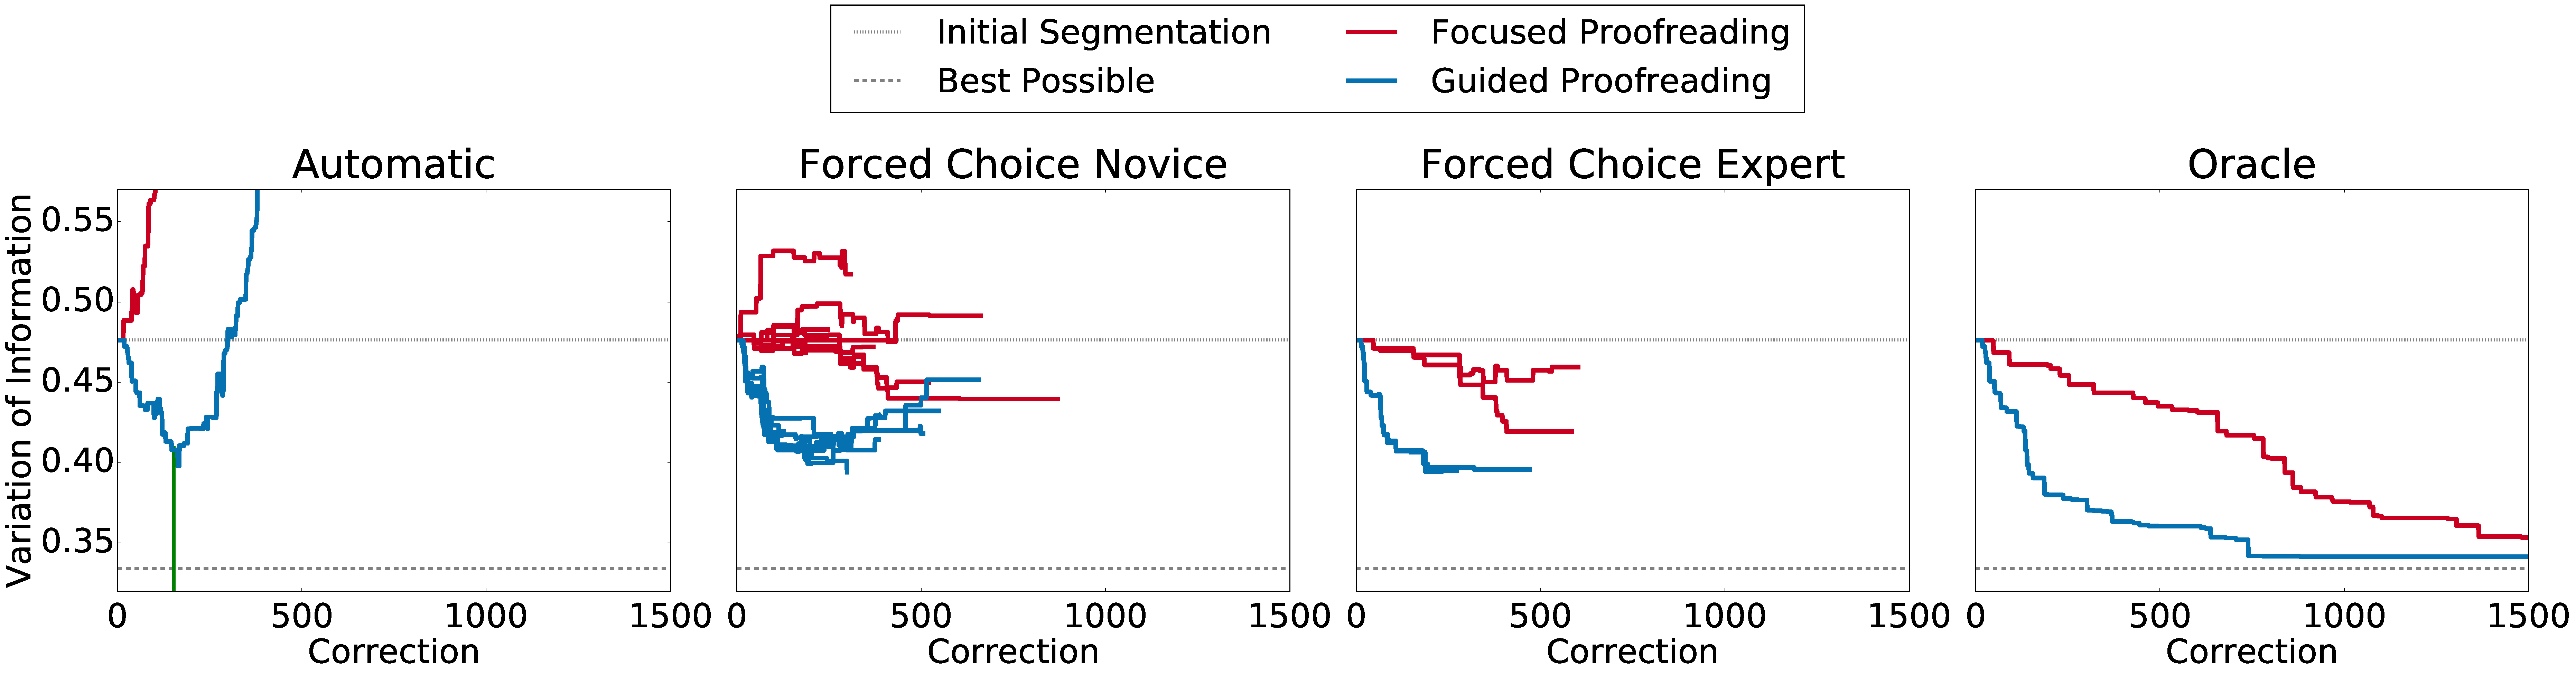
\includegraphics[width=\linewidth]{ac4trails_combined.pdf}
\caption{Performance comparison of Plaza's focused proofreading (red) and our guided proofreading (blue) on the AC4 subvolume. All measurements are reported as median VI, the lower the better. We compare different approaches of accepting or rejecting corrections for each method: automatic selection with threshold (green line), forced choice by ten novice users, forced choice by two domain experts, and the selection oracle. In all cases, guided proofreading yields better results with fewer corrections.}
\label{fig:ac4trails}
\end{figure*}

\paragraph{Expert study design.} We recruited 4 domain experts to evaluate the performance of both guided and focused proofreading. We obtained study consent and randomly assigned 2 experts to proofread using each classifier. The experts performed the 3 minute test run on different data prior to proofreading for 30 minutes. After the task ended, the experts were asked to complete the raw NASA-TLX questionnaire.

\paragraph{Evaluation metric.} We measure the similarity between proofread segmentations and the manual `ground truth' labelings using \textit{variation of information} (VI). VI is a measure of the distance between two clusterings, closely related to mutual information (the lower, the better).
